\documentclass[border=10pt]{standalone}

\usepackage{tikz}
\usepackage{tikzsymbols}
\usetikzlibrary{calc,patterns,shapes.geometric}

\def\centerarc[#1](#2)(#3:#4:#5){\draw[#1] ($(#2)+({#5*cos(#3)},{#5*sin(#3)})$) arc (#3:#4:#5);}

\begin{document}
	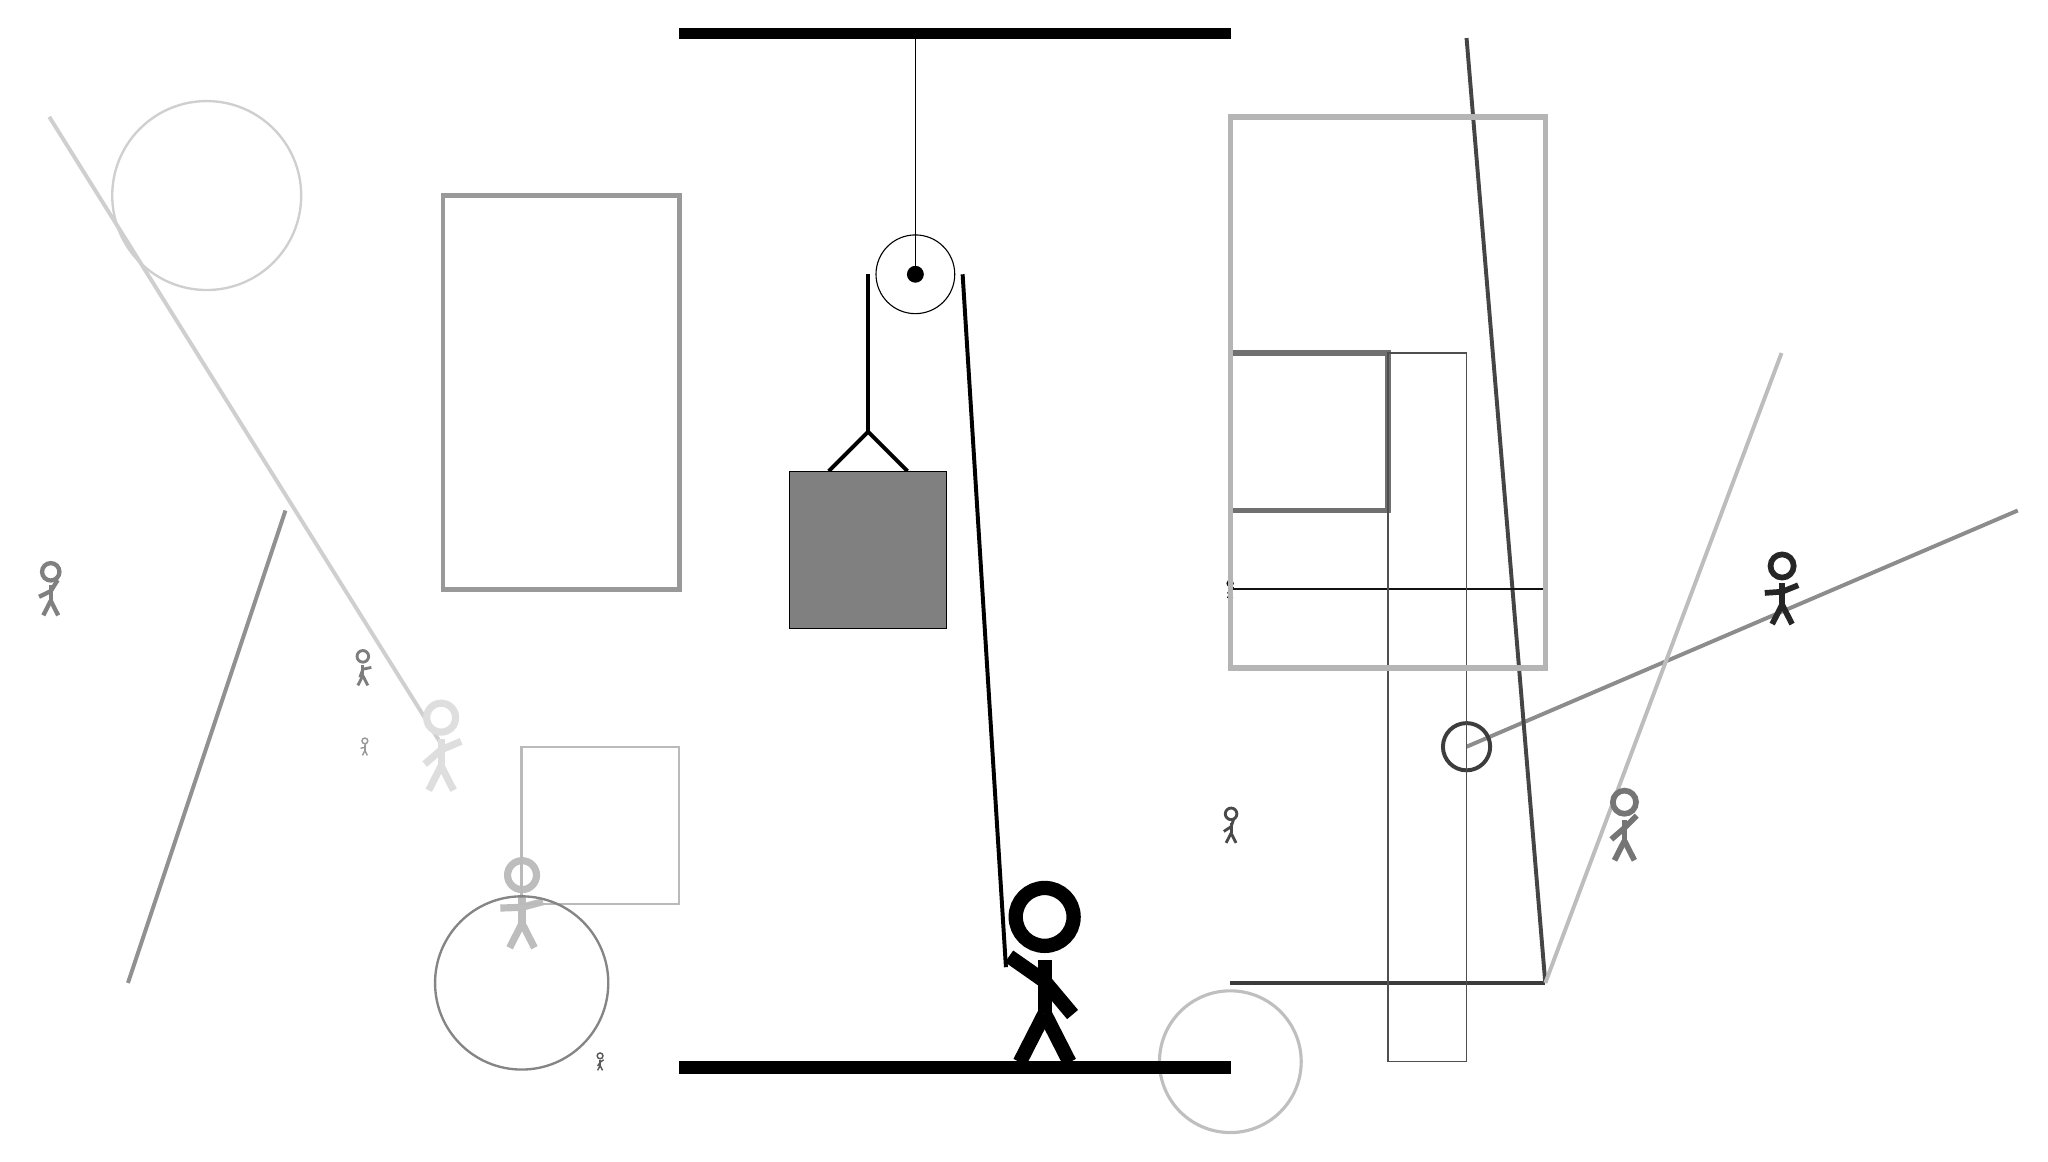
\begin{tikzpicture}
		%%%%% START %%%%%
		
		\draw[fill=black] (-2, 10) rectangle (5, 10.125);
		
		\draw (1, 7) circle (0.5);
		\draw[fill=black] (1, 7) circle (0.1);
		\draw (1, 10) -- (1, 7);
		
		\draw[line width=0.5mm] (-0.1, 4.5) -- (0.4, 5.0) -- (0.9, 4.5);
		\draw[fill=black!50] (-0.6, 4.5) rectangle (1.4, 2.5);
		
		\draw[line width=0.5mm] (0.4, 7) -- (0.4, 5.0);
		\centerarc[line width=0.5mm](1, 7)(0:180:0.6);
		\draw[line width=0.5mm](1.6, 7) -- (2.15, -1.8);
		
		\node at (2.6, -1.9) {\Strichmaxerl[10][-35][-50]};
		
		\draw[line width=0.5mm, color=black!45](8, 1) -- (15, 4);
		
		\node[line width=0.4mm, color=black!50] at (-10, 3) {\Strichmaxerl[3][26][58]};
		\node[line width=0.5mm, color=black!51] at (-6, 2) {\Strichmaxerl[2][70][12]};
		\node[line width=0.5mm, color=black!26] at (-4, -1) {\Strichmaxerl[5][2][15]};
		\draw [line width=0.3mm, color=black!19](-8, 8) circle (1.2);
		
		\draw[line width=0.5mm, color=black!73](9, -2) -- (8, 10);
		\draw[line width=0.5mm, color=black!43](-7, 4) -- (-9, -2);
		
		\node[line width=0.7mm, color=black!65] at (-3, -3) {\Strichmaxerl[1][56][35]};
		\draw[line width=0.7mm, color=black!56] (7, 4) rectangle (5, 6);
		\node[line width=0.2mm, color=black!85] at (12, 3) {\Strichmaxerl[4][4][22]};
		\draw[line width=0.5mm, color=black!77](5, -2) -- (9, -2);
		\node[line width=0.6mm, color=black!40] at (-6, 1) {\Strichmaxerl[1][12][79]};
		\draw[line width=0.5mm, color=black!26](9, -2) -- (12, 6);
		\draw [line width=0.5mm, color=black!76](8, 1) circle (0.3);
		\draw[line width=0.3mm, color=black!27] (-4, -1) rectangle (-2, 1);
		\draw[line width=0.5mm, color=black!19](-5, 1) -- (-10, 9);
		
		\node[line width=0.4mm, color=black!97] at (5, 3) {\Strichmaxerl[1][56][40]};
		\draw[line width=0.2mm, color=black!93] (5, 9) rectangle (9, 3);
		\draw [line width=0.3mm, color=black!48](-4, -2) circle (1.1);
		\node[line width=0.6mm, color=black!13] at (-5, 1) {\Strichmaxerl[5][41][23]};
		\draw[line width=0.2mm, color=black!69] (7, -3) rectangle (8, 6);
		
		\draw[line width=0.7mm, color=black!29] (5, 2) rectangle (9, 9);
		
		\draw [line width=0.4mm, color=black!25](5, -3) circle (0.9);
		\node[line width=0.7mm, color=black!71] at (5, 0) {\Strichmaxerl[2][33][71]};
		\node[line width=0.3mm, color=black!54] at (10, 0) {\Strichmaxerl[4][41][45]};
		
		\draw[line width=0.6mm, color=black!40] (-2, 8) rectangle (-5, 3);
		
		\draw[fill=black] (-2, -3) rectangle (5, -3.15);
		
		%%%%% END %%%%%
	\end{tikzpicture}
\end{document}